

\subsection*{Problem 1.5}
For each time iteration, the desired attitude $\mathbf{q}_d(t)$ given by $\phi(t) = 10sin(0.1t), \theta(t) = 0, \psi(t) = 15cos(0.05t)$, was converted to radians and then converted to quaternions by the use of the MATLAB function \texttt{euler2q()}. This was then conjugated and cross multiplied with the current $\mathbf{q}$ iteration by the use of the MATLAB functions \texttt{quatconj()} and \texttt{quatmultiply()} respectively. By doing so, $\mathbf{\tilde{q}}$ was calculated as per equation \eqref{eq:q_tilde}.

The $\tilde{\epsilon}$ part of $\mathbf{\tilde{q}}$ was extracted and combined with $\omega$ to create the state vector and was multiplied with the $\mathbf{K}$ \todo{referer til der K er skrevet!}to create the control input in the same way as in {\color{blue} attitude1.m}. The initial values were kept the same as previously and the $k_p$ and $k_d$ were changed to 10 and 300 respectively. 

\subsubsection*{Simulation results}

The simulation resulted in the plots given in \Cref{fig:sim_attitude2_euler} and \Cref{fig:sim_attitude2_track}.

\begin{figure}
	\centering
	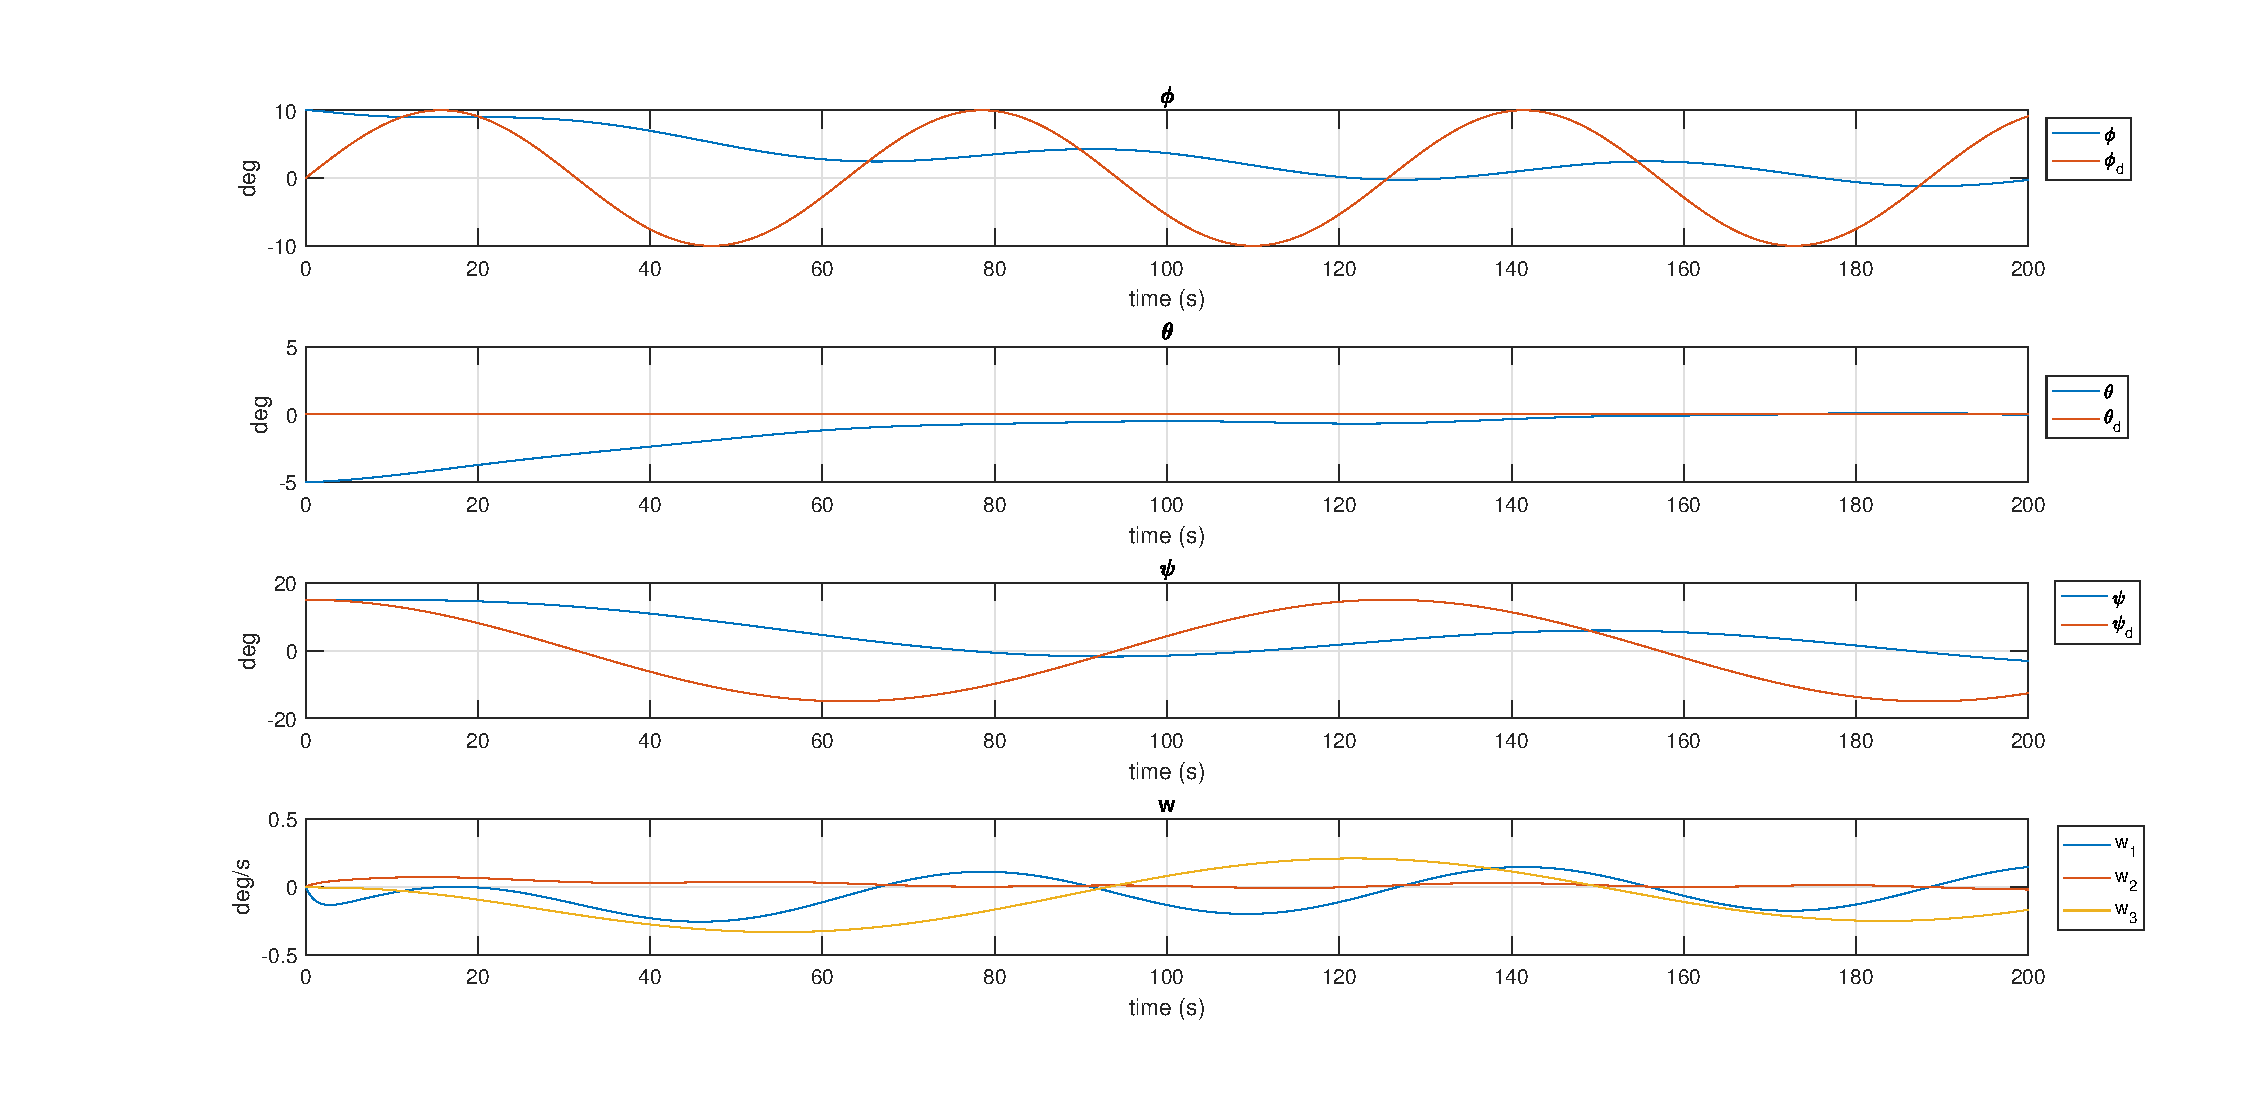
\includegraphics[width=1.00\textwidth]{figures/2_euler.eps}
	\caption{The resulting output euler angles with their corresponding desired values and the resulting output $\omega$ (denoted $\mathbf{w}$ in the plot) from the simulation in attitude2.}
\label{fig:sim_attitude2_euler}
\end{figure}

\begin{figure}
	\centering
	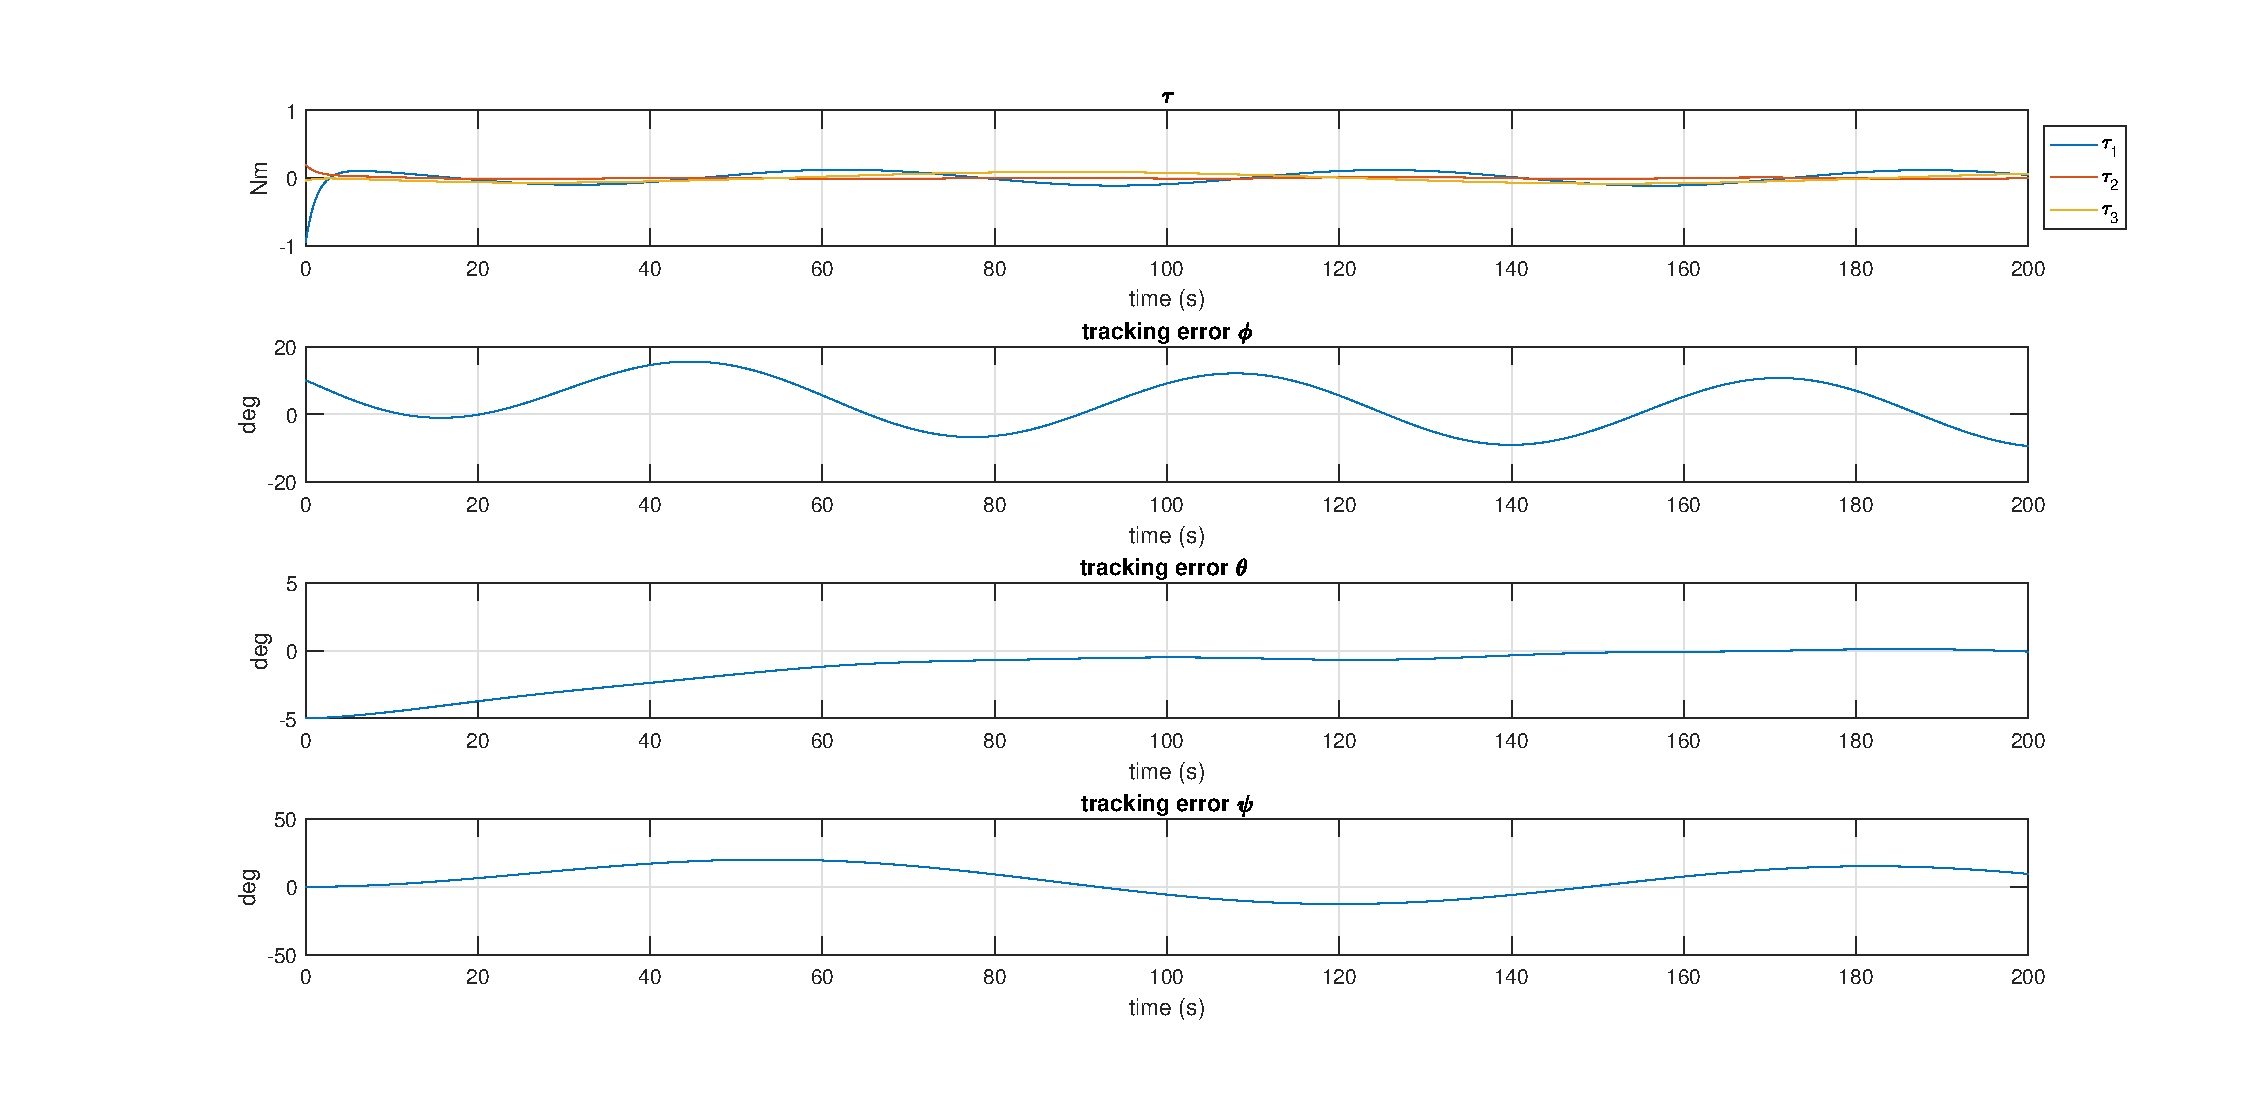
\includegraphics[width=1.00\textwidth]{figures/2_tau_track.eps}
	\caption{ $\tau$, and the tracking errors of the output euler angles from the simulation in attitude2.}
\label{fig:sim_attitude2_track}
\end{figure}

The Figures show that, with the exception of $\theta$, the angles of the satellite are following a sinusoidal pattern as per their desired values. However, they are not in sync with the desired signal and the amplitude is far too low compared to their intended forms, resulting in relatively large sinusoidal tracking errors as can be seen in \Cref{fig:sim_attitude2_track}. One reason for this misbehaviour is the fact that, even though the angles of the satellite is set to move in a specific way, the desired value of $\omega$ is still set to 0. This makes for a contradiction in the controller where neither part is able to do as they are told. The exception is $\theta$ and $\omega_1$ who are both set to 0.

It is also worth mentioning that the $\mathbf{K}$ matrix used for the controller was found using the linearized version of the system. This may also introduce errors.

\subsection*{Problem 1.6}

The attitude control law was modified to:
\begin{equation}
    \tau = -\mathbf{K}_d\tilde{\omega} -k_p\tilde{\epsilon}
    \label{eq:control_law_attitude3}
\end{equation}
\todo{Skal omega være i bold? Det er  ikke det i oppgaveteksten}

with $\tilde{\omega} = \omega - \omega_d$. Differentiating the desired attitude, $\Theta_d$, from the previous problem and calculating $\omega_d$ as

\begin{equation}
    \omega_d = \mathbf{T}_{\Theta_d}^{-1}(\Theta_d)\dot{\Theta_d}
    \label{eq:omega_d}
\end{equation}

We used the MATLAB function \texttt{eulerang()} to get the $\mathbf{T}_{\Theta_d}$ and set $k_p$ and $k_d$ to 10 and 300 respectively as before and used the $\omega_d$ calculated from \eqref{eq:omega_d} in the new simulation {\color{blue} attitude3.m}.

\subsubsection*{Simulation results}

We can see from \Cref{fig:sim_attitude3_euler} that the satellite is now able to follow the given reference signal in both angles and angle velocities. From \Cref{fig:sim_attitude3_track} we can see that though there still is an error in the $\phi$ and $\psi$ they are much smaller than previously. Now that $\omega$ and $\epsilon$ have corresponding desired values, they can both be satisfied by the same actions. The cooperation between the two parts of the state, which are in themselves related, is key to making a good controller. The linearization error discussed in the previous problem may still endure, but all in all the satellite control is much better than before.

\begin{figure}
	\centering
	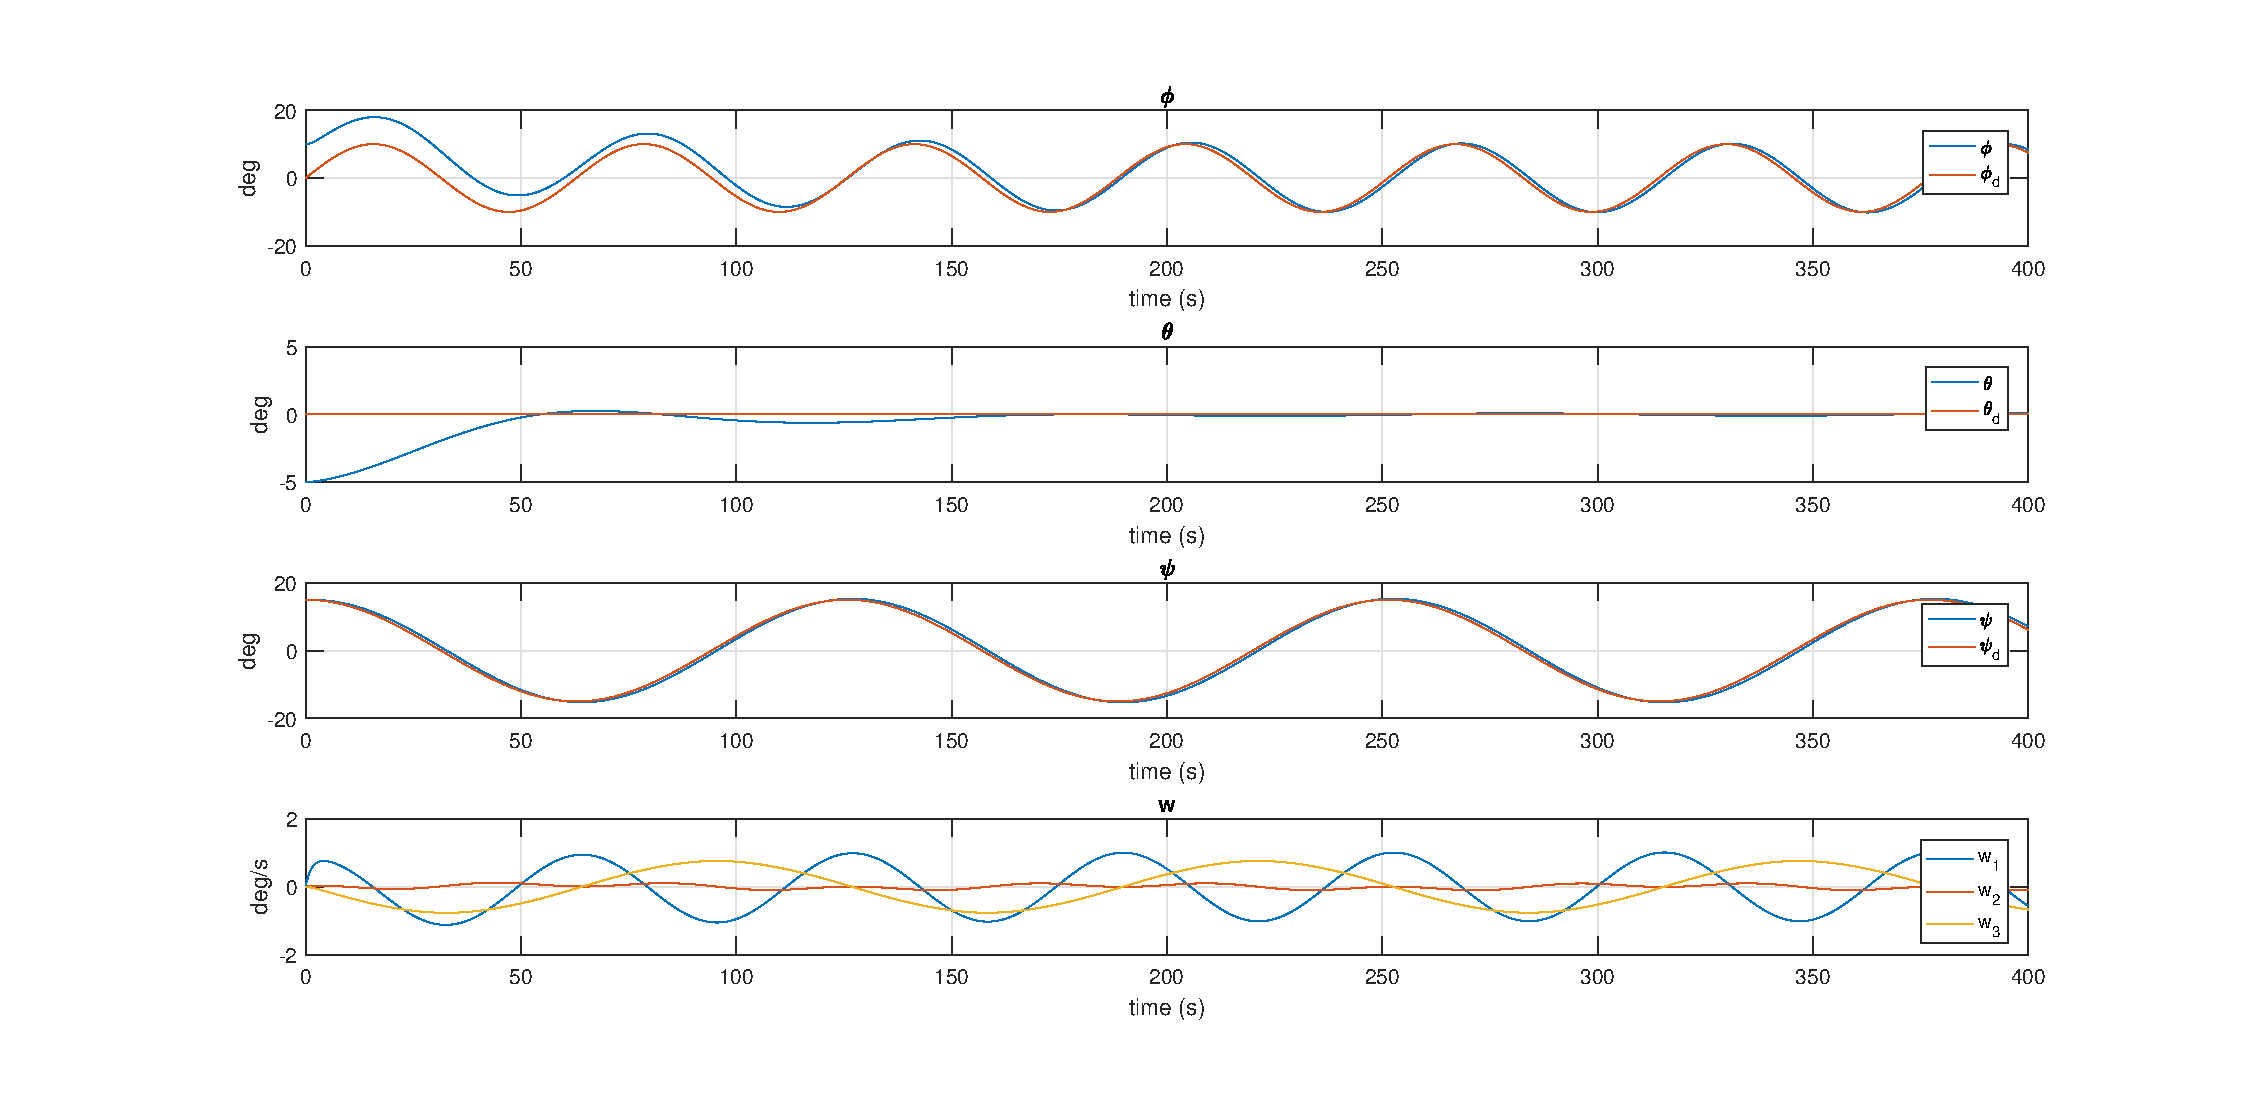
\includegraphics[width=1.00\textwidth]{figures/3_euler.eps}
	\caption{The resulting output euler angles with their corresponding desired values from the simulation in attitude3.}
\label{fig:sim_attitude3_euler}
\end{figure}

\begin{figure}
	\centering
	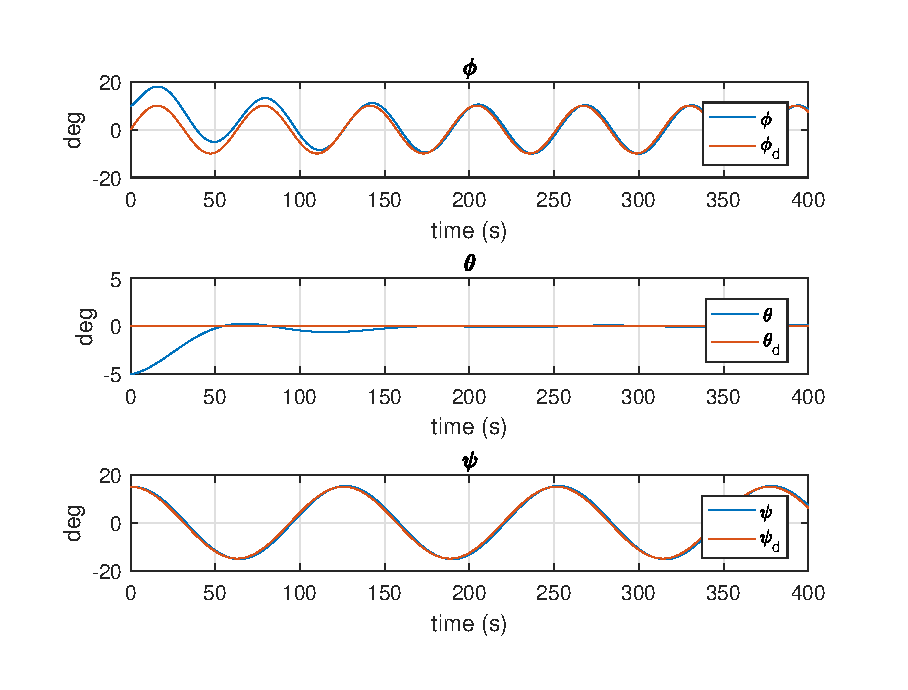
\includegraphics[width=1.00\textwidth]{figures/3_omega.eps}
	\caption{The resulting output $\omega$ (denoted $\mathbf{w}$ in the plots) and the corresponding desired values from the simulation in attitude3.}
\label{fig:sim_attitude3_omega}
\end{figure}

\begin{figure}
	\centering
	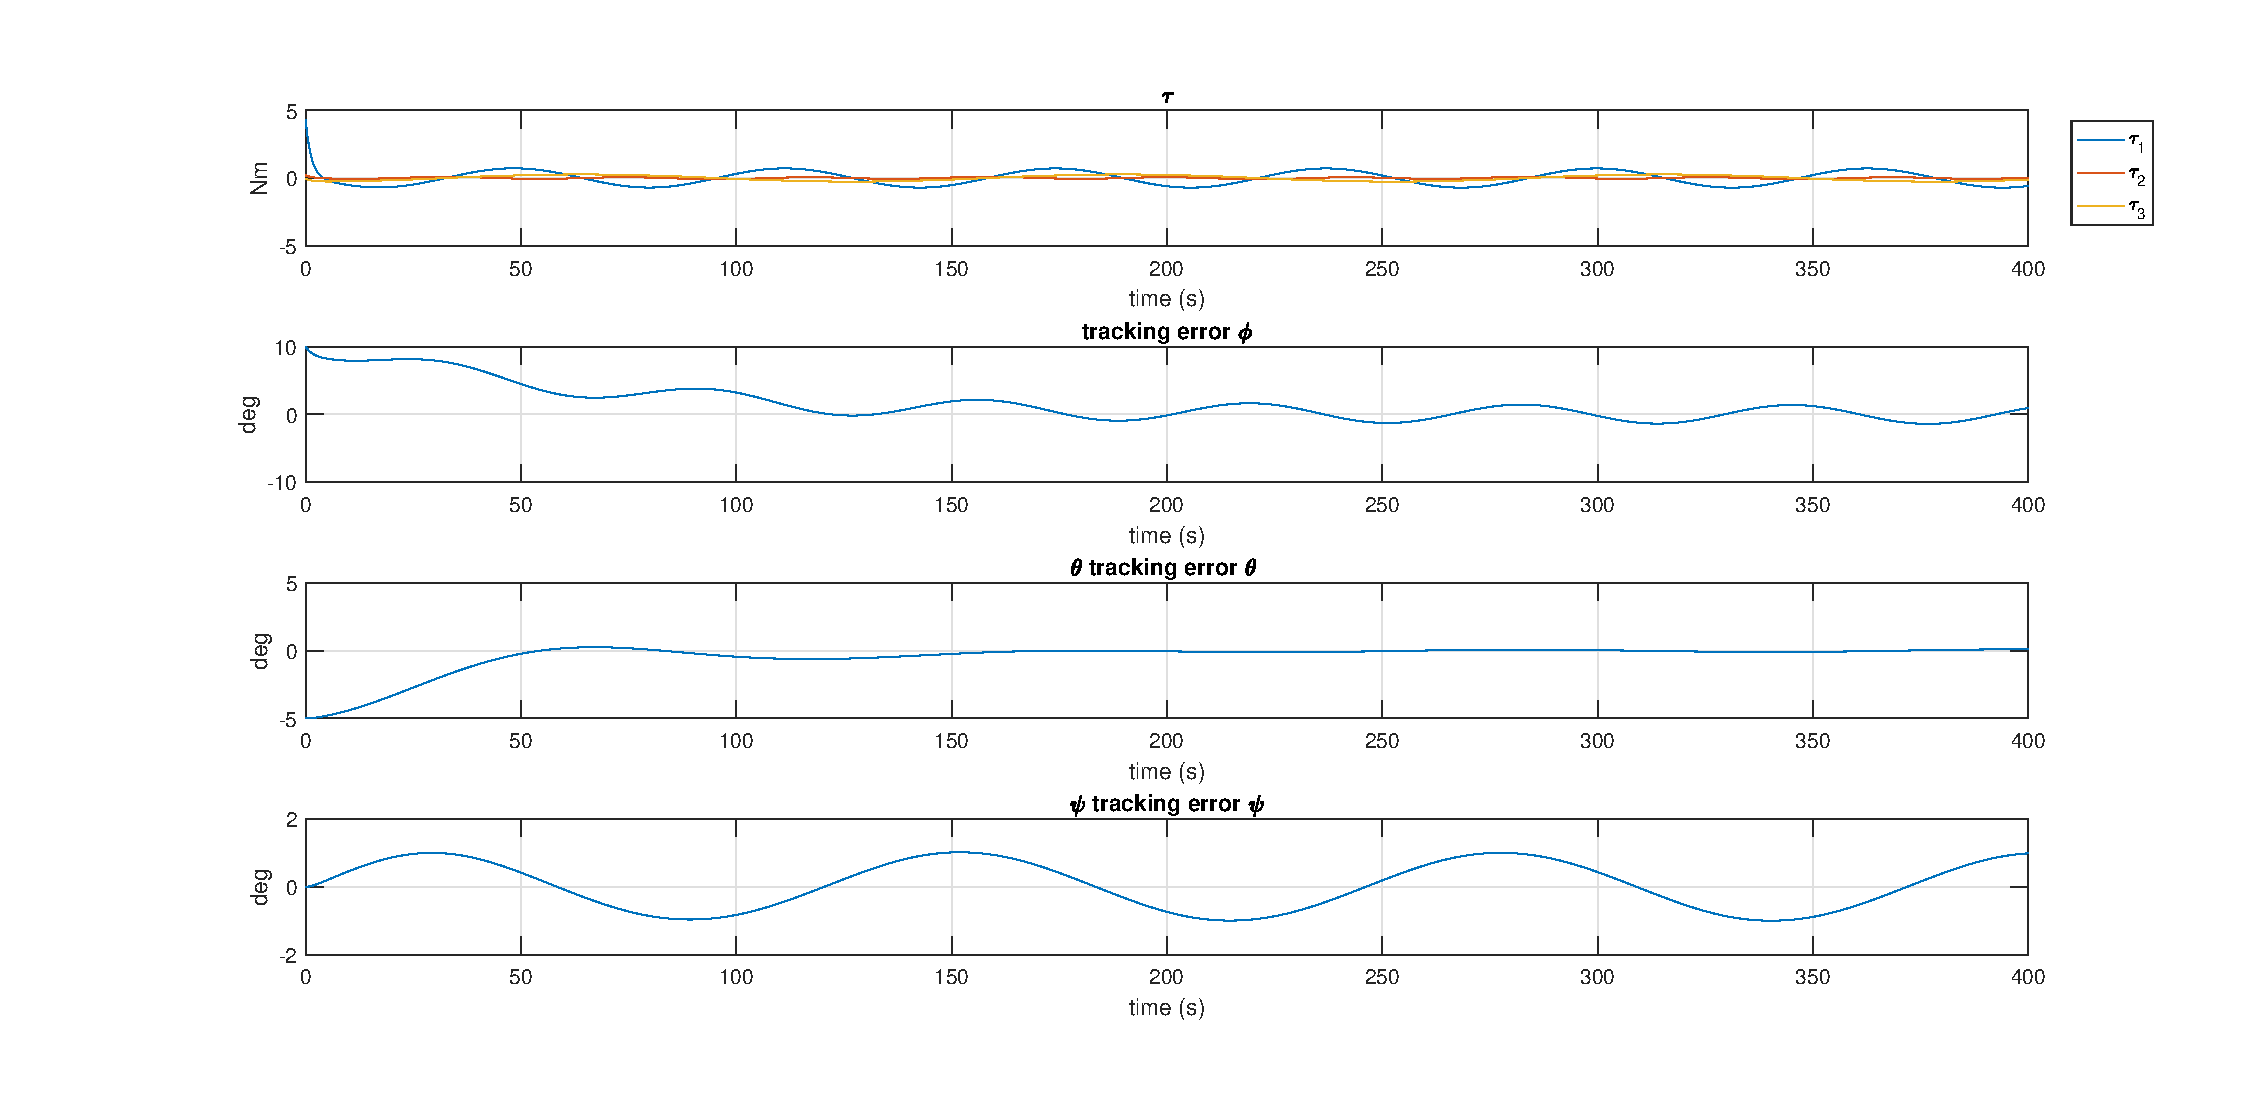
\includegraphics[width=1.00\textwidth]{figures/3_tau_track.eps}
	\caption{ $\tau$, and the tracking errors of the output euler angles from the simulation in attitude3.}
\label{fig:sim_attitude3_track}
\end{figure}

\subsection*{Problem 1.7}
Assuming $\omega_d = 0$ and $\epsilon_d$ and $\eta_d$ constants and the control law given by \eqref{eq:control_law_attitude2}, the Lyapunov function 
 \begin{equation}
	 V = \frac{1}{2} \tilde{\boldsymbol{\omega}}^{\top} \mathbf{I}_{CG}\tilde{\boldsymbol{\omega}} + 2 k_p (1-\tilde{\eta})
 \end{equation}
 
is positive and radially unbounded. 

The reason for its positivity is that $\mathbf{I}_{CG}$ being an identity matrix with a positive number, $mr^2$, on its diagonal, is positive definite. So the first part of V is positive (labeling 0 as a positive number). The second part, consisting of $2 k_p (1-\tilde{\eta})$, may only be negative if $\tilde{\eta} > 1$. This will never happen however, as $\tilde{\eta}$ is part of the unit quaternion $\tilde{q}$ making $|\tilde{\eta}| \leq 1$. Thus the second part of V will also be positive. The Lyapunov function is usually thought of as a representation of the energy in the system so the fact that it is never negative makes sense. 

The function is radially unbounded 

\subsection*{Problem 1.8}
...

% Note that \mathbf can be used for bold letters in math mode (within equations and dollar signs). \boldsymbol can be used to get bold greek letters.  

